\section{Methods: The MINI pipeline}

\begin{figure}[h]
    \centering
    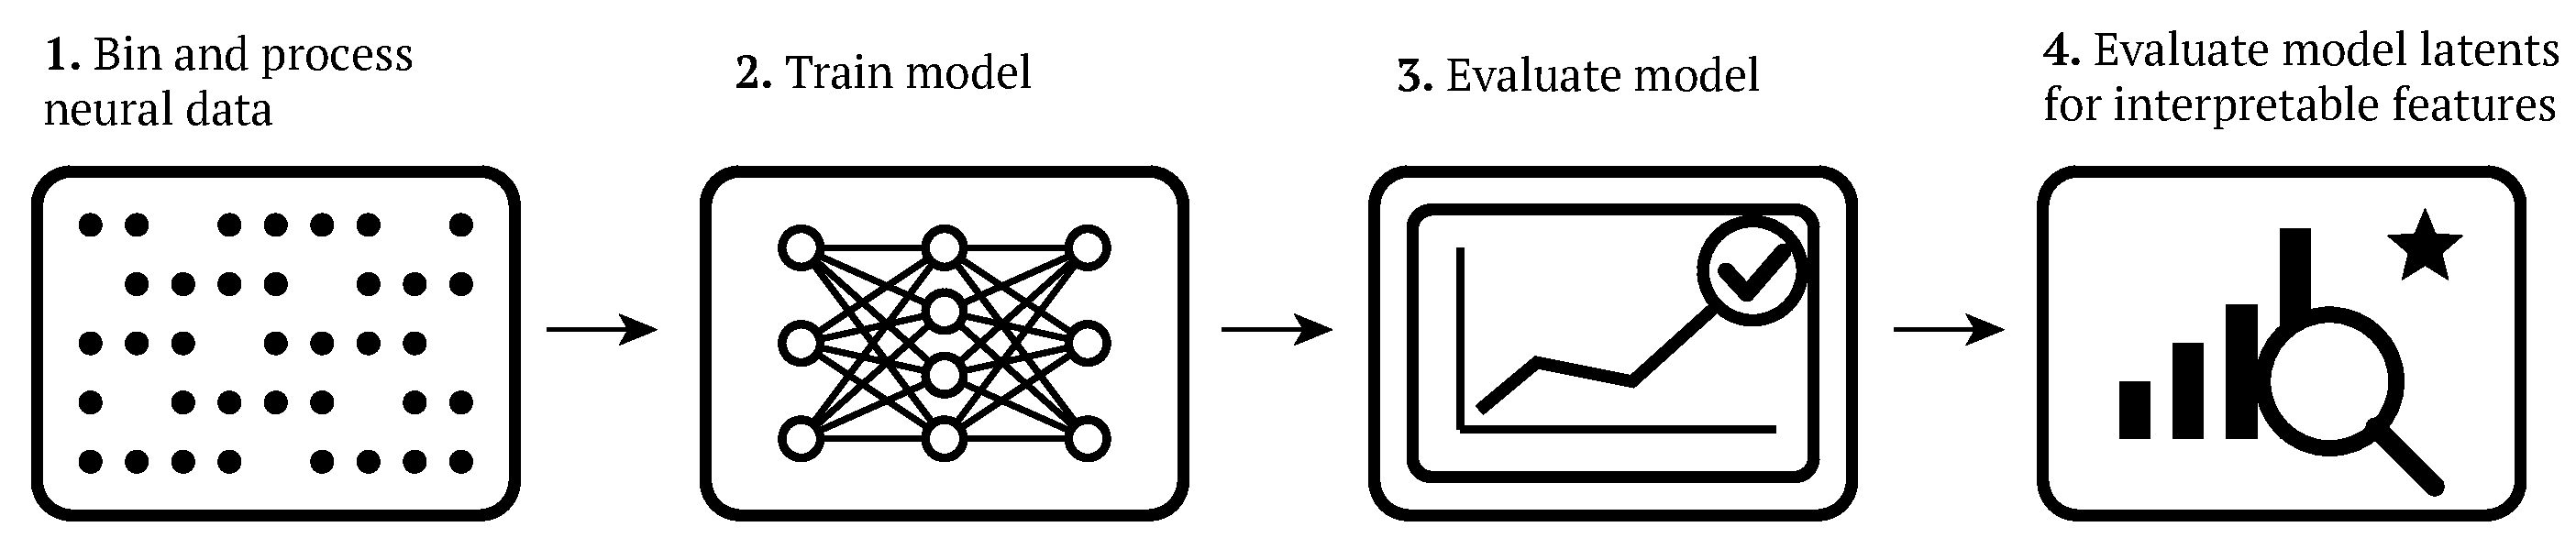
\includegraphics[width=\linewidth]{figures/mini_pipeline.pdf}
    \caption{
        \textbf{The MINI pipeline.} \\
        \small The MINI pipeline is comprised of 4 stages: 1) Spatiotemporal binning and processing of neural data; 2) Model training; 3) Model evaluation; 4) Latent evaluation for feature interpretability. Steps 1-3 can be either semi- or fully-automated.
    }
    \label{fig:mini_pipeline}
\end{figure}

The MINI pipeline transforms high-dimensional neural data into a set of interpretable latents in four primary stages (\autoref{fig:mini_pipeline}), the first three of which can be fully automated.

\subsection{Data preprocessing}

The pipeline's first stage prepares neural data for model training. MINI includes utilities to process outputs from common spikesorters (e.g. Kilosort ~\cite{pachitariu_2016_kilosort}) by aggregating, binning, and normalizing spike times into a 2D matrix of time by space, in which each bin contains neural activity from a neural unit for a specific time period. Normalization operations include min-max and z-scoring, applied across either the spatial or temporal dimension. This processing is readily adaptable to other forms of acquired neural data, such as ROIs from calcium imaging data processed by tools like Suite2p ~\cite{pachitariu_2017_suite2p}. Alternatively, users may pass their own preprocessed neural data directly to the model training stage.

\subsection{Model training}

In stage 2, a SDNN model is trained to reconstruct the processed neural data from latent, sparsely active dictionary elements -- the model's hidden layer neurons\footnote{In a SDNN model: model neuron = dictionary element = latent}. The end goal is for these latents to represent disentangled, interpretable representations\footnote{In our vernacular: interpretable latent $\approx$ feature $\approx$ representation} encoded by the neural activity (\autoref{fig:sdnn_arch}\textbf{a},\textbf{b}). The sparsity encourages the model to discover a monosemantic dictionary, in which each latent corresponds to a single feature. For instance, a latent from a model trained on visual cortex activity may correspond to a particular property of a visual stimulus, while a latent from a model trained on motor cortex activity may correspond to a specific aspect of movement.

The model can be configured as an autoencoder, transcoder, or crosscoder ~\cite{lindsey_2024_crosscoders}, depending on the relationship between the input and target neural data. As an autoencoder, the model reconstructs its own input; e.g. reconstructing V1 activity based on V1 activity. As a transcoder, the model reconstructs a dependent target from a different input; e.g. reconstructing V2 activity based on V1 activity. As a crosscoder, the model reconstructs a related target of a different input; e.g. reconstructing V1 activity on day 2 based on V1 activity on day 1. In all cases, the model is trained to minimize the difference between the reconstructed and actual target neural data. The training procedure is summarized here:

\begin{algorithm}[h!]
\caption{MINI Training Procedure}
\label{alg:mini_training}
\begin{algorithmic}[1]
\State \textbf{Define Inputs:}
\State \quad Input neural data: $\mathbf{X}_{\text{in}} \in \mathbb{R}^{B \times S \times N_{\text{in}}}$ (Batch, Sequence, Input Neurons)
\State \quad Target neural data: $\mathbf{X}_{\text{target}} \in \mathbb{R}^{B \times S \times N_{\text{out}}}$ (Batch, Sequence, Output Neurons)
\State \textbf{Define Model Parameters} $\theta$:
\State \quad Encoder: $\mathbf{W}_{\text{enc}} \in \mathbb{R}^{D_{\text{max}} \times (S \cdot N_{\text{in}})}$, $\mathbf{b}_{\text{enc}} \in \mathbb{R}^{D_{\text{max}}}$
\State \quad Decoder: $\mathbf{W}_{\text{dec}} \in \mathbb{R}^{(S \cdot N_{\text{out}}) \times D_{\text{max}}}$, $\mathbf{b}_{\text{dec}} \in \mathbb{R}^{S \cdot N_{\text{out}}}$
\State \quad Self-Attention (optional): $\theta_{\text{attn}}$
\State \textbf{Define Hyperparameters:}
\State \quad Matryoshka levels $\{D_l\}_{l=1}^L$, Reconstruction loss weights $\{\lambda_l\}_{l=1}^L$, Auxiliary loss weight $\gamma$
\Procedure{TrainStep}{$\mathbf{x}_{\text{in}}, \mathbf{x}_{\text{target}}$}
    \State $\mathbf{x}_{\text{in}} \gets \text{Reshape}(\mathbf{x}_{\text{in}}, [B, S \cdot N_{\text{in}}])$
    \State $\mathbf{x}_{\text{target}} \gets \text{Reshape}(\mathbf{x}_{\text{target}}, [B, S \cdot N_{\text{out}}])$
    
    \Statex \Comment{\textit{--- Forward Pass ---}}
    \State $\mathbf{A} \gets \text{ReLU}(\mathbf{x}_{\text{in}}\mathbf{W}_{\text{enc}}^T + \mathbf{b}_{\text{enc}})$ \Comment{Encoder Activations}
    \If{$S > 1$}
        \State $\mathbf{A} \gets \text{SelfAttention}(\mathbf{A}; \theta_{\text{attn}})$ \Comment{Temporal Integration}
    \EndIf

    \State $\mathcal{L}_{\text{recon}} \gets 0$
    \For{$l=1$ to $L$} \Comment{Multi-level Reconstruction}
        \State $\hat{\mathbf{A}}_l \gets S_{\text{topk}}(\mathbf{A}_{:, :D_l})$ \Comment{Batch Top-$k$ Sparsity}
        \State $\hat{\mathbf{x}}_l \gets \text{ReLU}(\hat{\mathbf{A}}_l \mathbf{W}_{\text{dec}, :, :D_l}^T + \mathbf{b}_{\text{dec}})$ \Comment{Reconstruction}
        \State $\mathcal{L}_{\text{recon}} \gets \mathcal{L}_{\text{recon}} + \lambda_l \cdot \text{MSE}(\mathbf{x}_{\text{target}}, \hat{\mathbf{x}}_l)$
    \EndFor
    
    \Statex \Comment{\textit{--- Auxiliary Loss for Dead Feature Resurrection ---}}
    \State $\mathcal{D} \gets \text{GetDeadFeatures}(\mathbf{A})$
    \State $\mathbf{r} \gets \mathbf{x}_{\text{target}} - \hat{\mathbf{x}}_L$ \Comment{Reconstruction Residual}
    \State $\hat{\mathbf{r}} \gets \text{ReLU}((\mathbf{A} \odot \mathcal{D}) \mathbf{W}_{\text{dec}}^T + \mathbf{b}_{\text{dec}})$ \Comment{Reconstruct residual from dead features}
    \State $\mathcal{L}_{\text{aux}} \gets \text{MSE}(\mathbf{r}, \hat{\mathbf{r}})$
    
    \State $\mathcal{L}_{\text{total}} \gets \mathcal{L}_{\text{recon}} + \gamma \mathcal{L}_{\text{aux}}$
    
    \Statex \Comment{\textit{--- Backward Pass \& Parameter Update ---}}
    \State $\mathbf{g} \gets \nabla_{\theta} \mathcal{L}_{\text{total}}$ \Comment{Compute gradients, masking $\nabla\mathcal{L}_{\text{aux}}$ to dead features}
    \State $\theta \gets \text{AdamUpdate}(\theta, \mathbf{g})$ \Comment{Update model parameters}
\EndProcedure
\end{algorithmic}
\end{algorithm}

\paragraph{Matryoshka Architecture.}
As shown in Algorithm \ref{alg:mini_training}, we train the model to reconstruct target activity from multiple, nested dictionaries simultaneously. This Matryoshka structure \cite{bussmann_2025_msae} encourages the discovery of a multi-scale feature representation. Because each dictionary level $D_l$ is responsible for a full reconstruction, smaller dictionaries learn coarse, high-variance features, while larger ones learn progressively finer-grained features that explain the remaining variance.

\paragraph{Batch Top-$k$ Sparsity.}
Sparsity is enforced using a batch top-$k$ operator, $S_{\text{topk}}(\cdot)$, which preserves only the $k \cdot B$ features with the highest activation magnitude across a batch of size $B$. This approach directly controls feature sparsity without introducing a tunable regularization coefficient (e.g., for an L1 penalty). Furthermore, it permits the number of active features per individual sample to vary, a flexible property that aligns well with the variable complexity of neural states.

\paragraph{Temporal Integration with Self-Attention.}
When input data is provided as a sequence ($S>1$), an optional self-attention layer integrates information across the feature activation dimension (supplementary fig). This mechanism allows the model to learn features corresponding to temporal dynamics and state transitions, moving beyond representations of purely instantaneous neural patterns.

\paragraph{Dead Feature Resurrection.}
A common failure mode in training autoencoders is "feature death," where dictionary elements cease to activate for any input. We address this with an auxiliary loss designed to revive dead features. We monitor feature activation frequencies and identify a set of dead features $\mathcal{D}$. These features are then trained via an auxiliary MSE loss to reconstruct the residual error of the primary model ($\mathbf{x}_{\text{target}} - \hat{\mathbf{x}}_L$). The gradients from this auxiliary loss are exclusively applied to the parameters of the dead features, thereby encouraging them to learn useful representations without disrupting the training of active features.

\begin{figure}[htbp]
    \begin{minipage}{0.63\linewidth}
    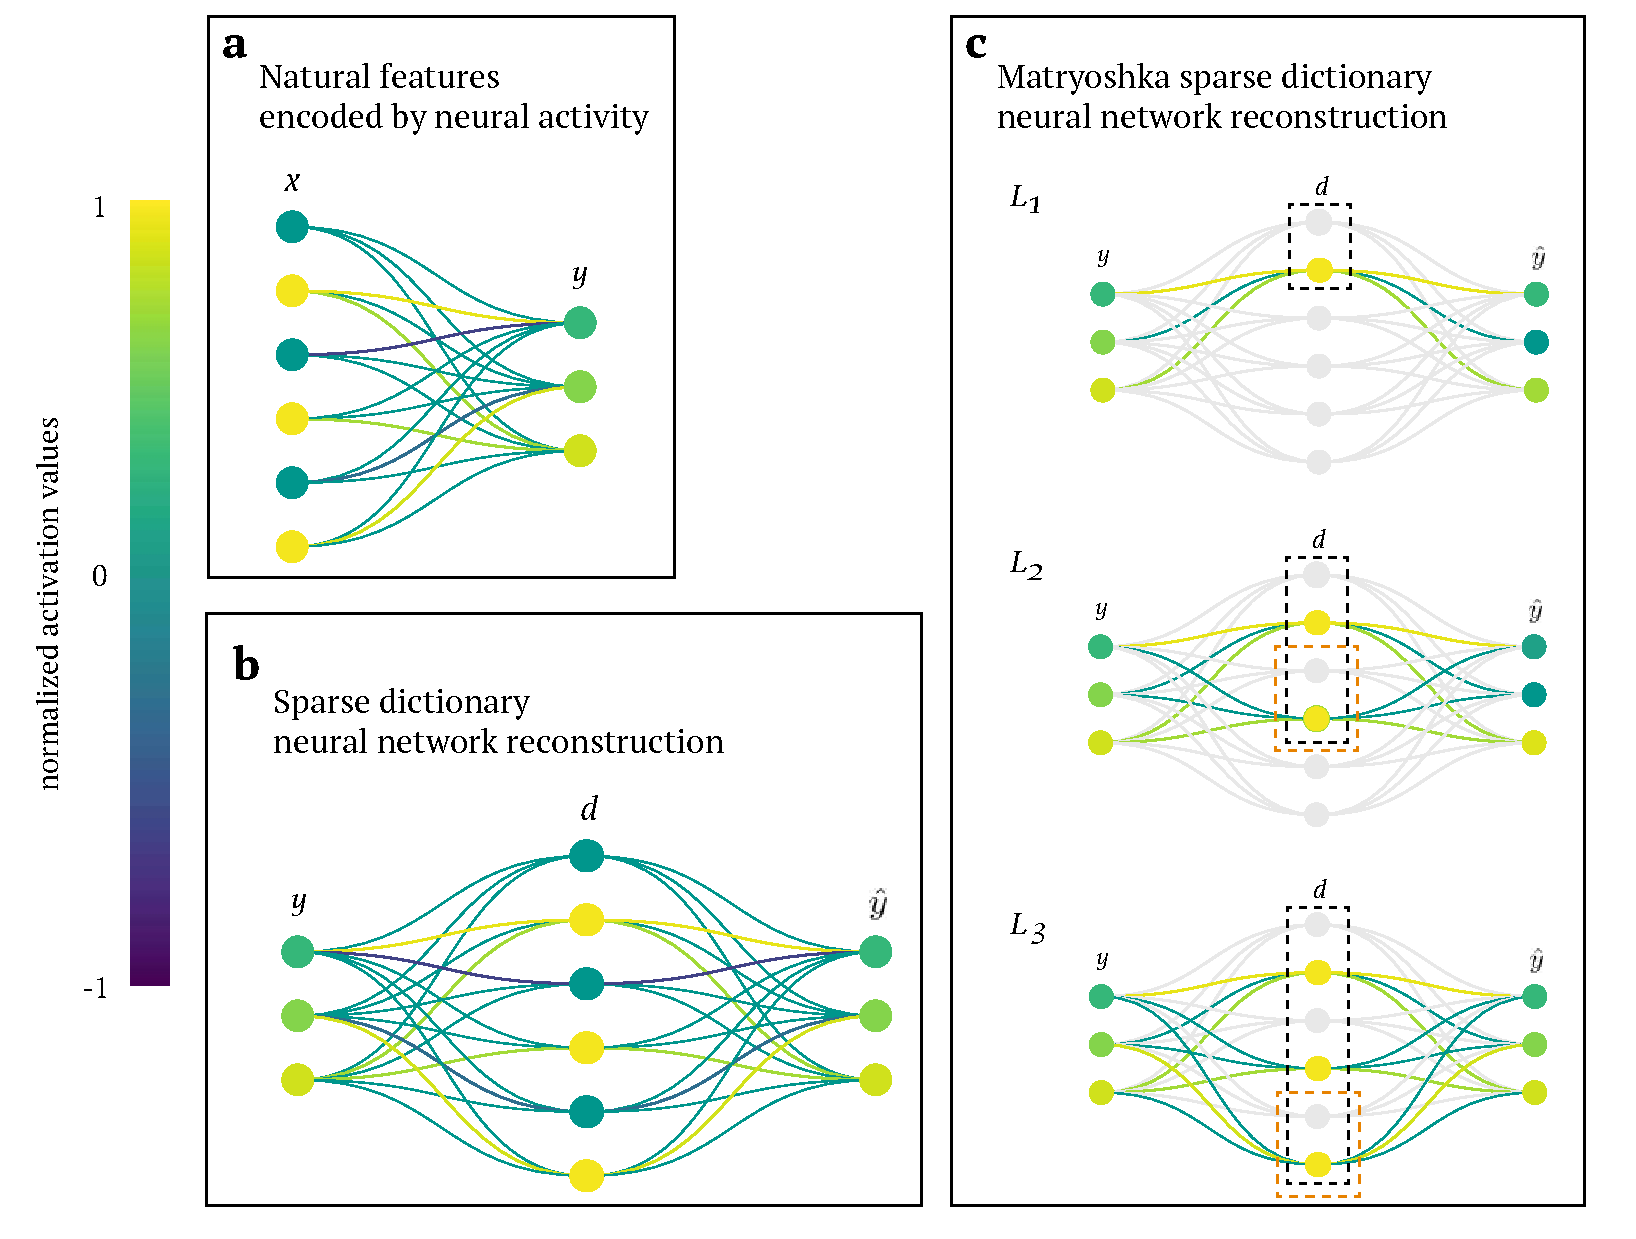
\includegraphics[width=\linewidth]{figures/sdnn_arch.pdf}
    \end{minipage}%
    \begin{minipage}{0.37\linewidth}
    \caption{
        \textbf{Model motivation} \\
        \small
        (\textbf{a}) Natural, "real-world" features $x$ are encoded by neural activity $y$. In this example, three active features are simultaneously represented by the joint activity of three neurons. (\textbf{b}) A SDNN reconstructs neural activity $z$ based on $y$ via sparse dictionary elements $d$. When training is successful, $d$ corresponds to $x$: sparse dictionary elements (i.e. model neurons) represent natural features. If $z$ tries to recreate $y$ exactly ($\hat{y}$), the model is an autoencoder; in other scenarios (e.g. $z$ is separate but dependent on or related to $y$) it is a transcoder or crosscoder. (\textbf{c}) A Matryoshka spare dictionary neural network segments the latent space into multiple levels, each of which attempts to do a full reconstruction of the target neural activity. The black boxes indicate the latents involved in a single level, while the light red boxes indicate the additional latents used at lower-levels. Additionally, for each level here we illustrate imposing a topk of 1 for each level, where only 1 latent (the most active) is chosen for reconstruction at each level. Latents in the highest-level will often correspond to high-level features (e.g. a round object), while latents exclusive to the lowest-level will often correspond to low-level features (e.g. a basketball).
    }
    \label{fig:sdnn_arch}
    \end{minipage}
\end{figure}

\hrule
\hrule

- MINI employs a novel variant of the Matryoshka SDNN architecture ~\cite{bussmann_2025_msae} to segment the latent space into multiple hierarchical levels, with each level attempting a full reconstruction of the target neural activity (\autoref{fig:sdnn_arch} \textbf{c}). This allows for multi-feature representation at a single point in time. e.g. we can have neural representations for a round object, a ball, and most specifically, a basketball, when we see one. With other approaches, we are more likely to see "feature absorption", where we cannot distinguish to features that have neural representations if one is a subset of the other.

- Compared to a vanilla Matryoshka SDNN architecture, we've found empirically that in some cases batch topk and the addition of the transformer layer to the decoder improves reconstruction and interpretability (additional results).

- Show latex formulas for encoder, decoder, total loss.

- Model training can be set to run with a sweep, after which multiple models are evaluated in the subsequent pipeline step. The common model hyperparameters to sweep over are n\_levels, dsae\_levels, topk, and latent space sequence length. Depending on the optimizer used, it's recommended to additionally sweep over hyperparameters such as learning rate (we use Adam by default bc...)

(For additional details on model architecture and training, see \nameref{subsection:additional_pipeline_details}.)

In step 3, the trained model is evaluated using a variety of metrics to assess its performance. (SAEBench) If the model does not meet the desired criteria, it can be re-trained with different hyperparameters. 

\begin{figure}[h]
    \centering
    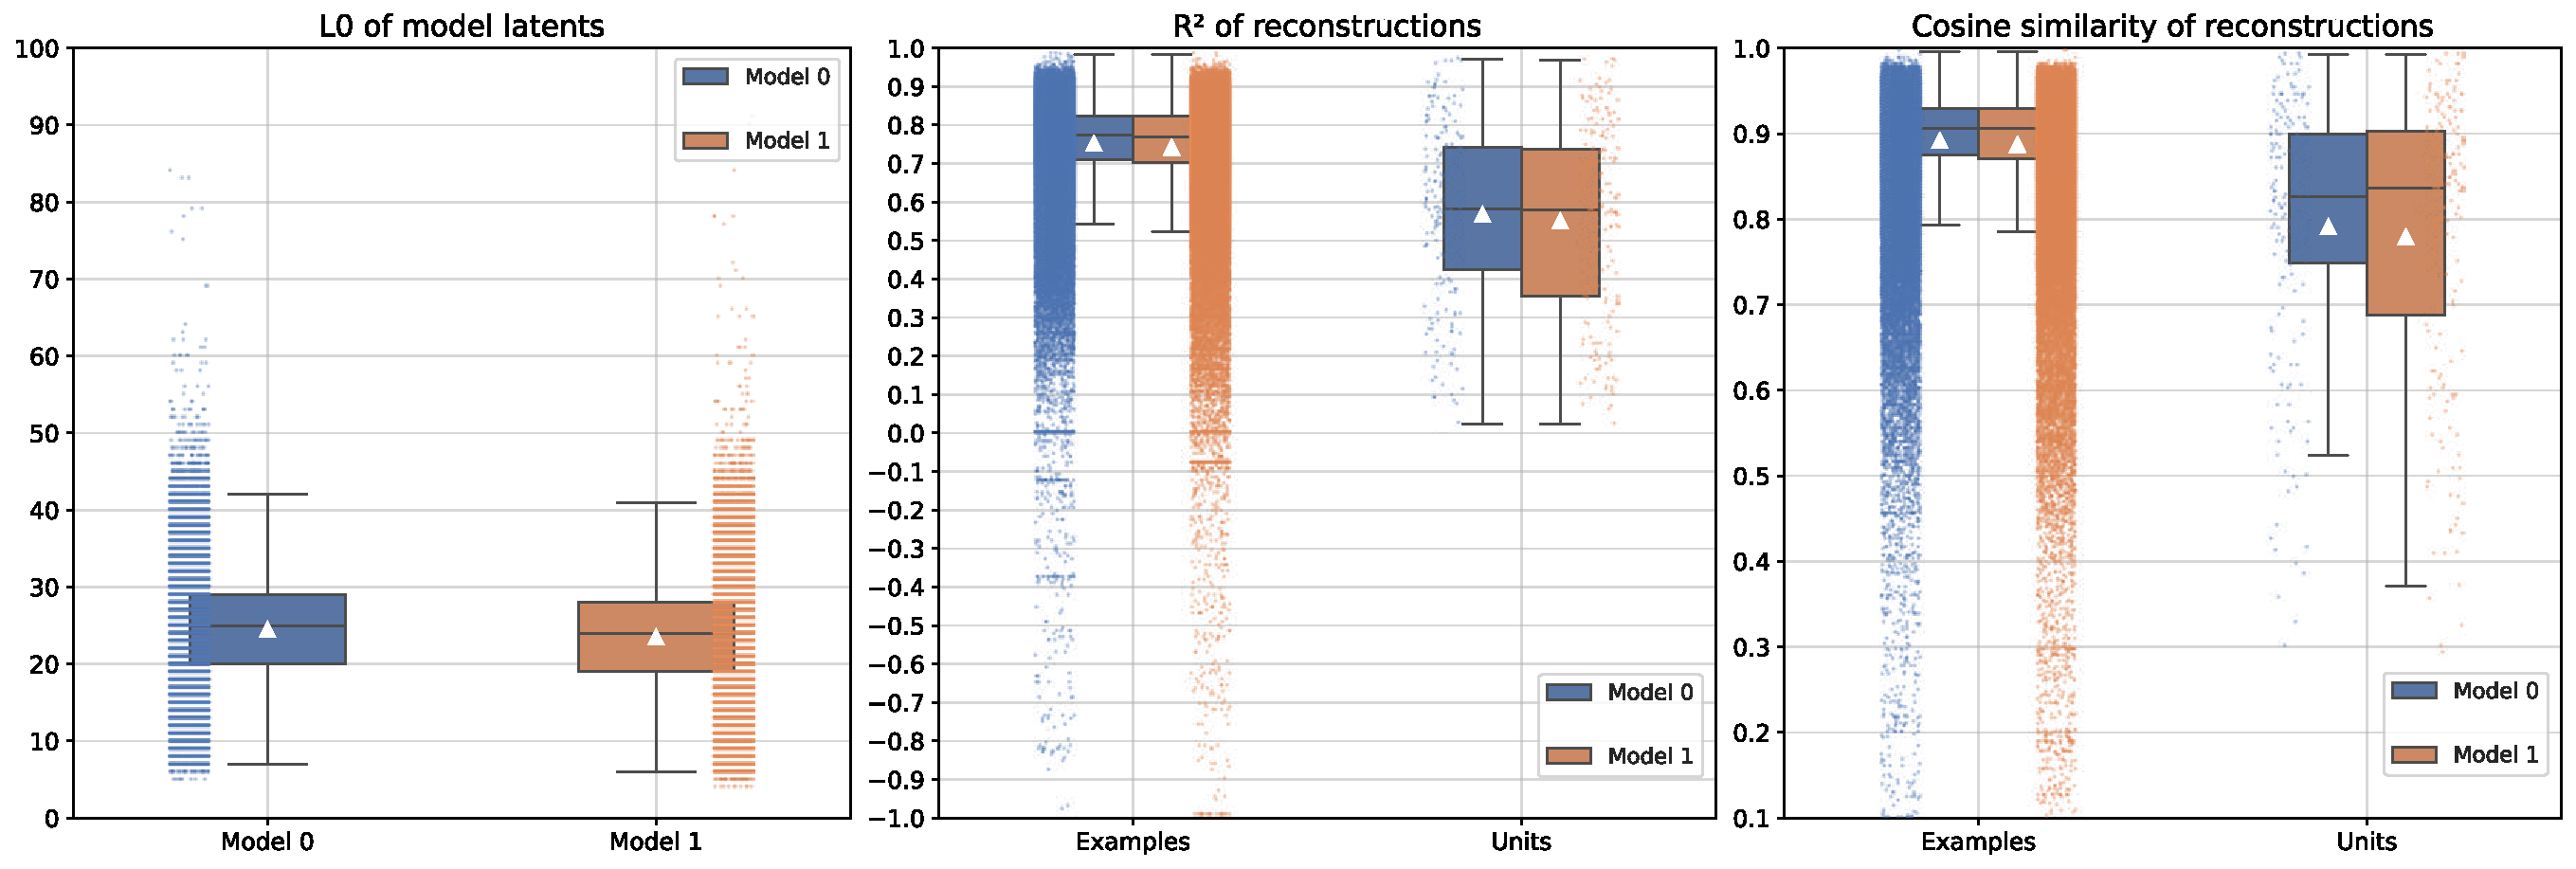
\includegraphics[width=\linewidth]{figures/model_eval.pdf}
    \caption{
        \textbf{Model evaluation metrics.} \\
        \small By default, trained models are evaluated via the following metrics: latent L0 (left), and R\textsuperscript{2} (middle) and cosine similarity (right) of reconstruction-to-actual neural activity for each temporal ("Examples") and spatial ("Units") bin. ... Additional features, such as the R\textsuperscript{2}of overall neural data reconstruction for each individual latent, can be specifed and included.
    }
    \label{fig:model_eval}
\end{figure}

Finally, in step 4, the latents produced by the model are evaluated for interpretability as features. This includes visualizing their activation patterns over time and experimental conditions, as well as assessing their decoding performance. We detail typical approaches to feature evaluation in \nameref{section:results}.

- For a user, the full, semi-automated pipeline is as follows:
\begin{enumerate}
    \item Data processing
    \begin{itemize}
        \item Spatiotemporally bin and normalize
        \begin{itemize}
            \item MINI has a convenience function to do this directly from output of common spikesorters (kilosort), where we bin unit spikes given a specified timebin and optionally normalize (z-score or max) dataset across time and/or unit
            \begin{itemize}
                \item (and similar approach could be applied to output from common calcium imaging processing (e.g. Suite2p))
            \end{itemize}
        \end{itemize}
    \end{itemize}
    
    \item Model training
    \begin{itemize}
        \item Hyperparameter optimization
        \begin{itemize}
            \item Model parameters
            \item Optimizer parameters
        \end{itemize}
        \item By default no validation set, but can be added if we want to e.g. apply to other recordings of same animal, though this is not generally recommended (just train a freshie)
    \end{itemize}
    
    \item Model evaluation
    \begin{itemize}
        \item (We implement all metrics from SAEBench which are not language-model specific, plus a couple of our own)
        \item L0 of latents
        \item R\textsuperscript{2} (var explained) and cos sim of reconstruction-to-actual neural activity for each spatial bin, and each temporal bin
        \item Latent density histogram (as in SAEBench)
        \item Variance explained of overall reconstruction from each latent (variance shouldn't be in just a few features) ?
        \item Spectral frequency analysis to ensure temporal frequency content is preserved?
    \end{itemize}
    
    \item Feature evaluation
    \begin{itemize}
        \item When a latent is subjectively determined to be sufficiently interpretable, we call this a feature.
        \item Interactive plots showing feature activation patterns across time and experimental conditions.
        \item We evaluate its decoding performance?
        \item Export functionality.
    \end{itemize}
\end{enumerate}


